\chapter{Burrows-Wheeler-Transformation}

Die \term{Burrows-Wheeler-Transformation}\index{Burrows-Wheeler-Transformation} erzeugt eine sinnvolle Permutation des eingegebenen Strings; sie gruppiert Zeichen mit ähnlichem Kontext nahe beieinander. Die Struktur der Permutation beinhaltet alle Informationen, die benötigt werden, um eine Rücktransformation durchzuführen, es sind also keine Zusatzinformationen nötig. Hin- und Rücktransformation geht in \( O(n) \). Sie wird hauptsächlich zur Vorverarbeitung statischer Texte genutzt, um sie komprimieren, indizieren und in ihnen suchen zu können.

\section{Konstruktion}

Sei \( T = \texttt{lalalangng\$} \) der gegebene String (mit angehängtem \$-Zeichen), \( n = \left\vert T \right\vert \) und \( T^{(i)} \) die \( i \)-te Permutation von \( T \) (durch \( i \) mal den vordersten Buchstaben nehmen und hinten anhängen). Man erhält die Burrows-Wheeler-Transformation von \( T \) so:

\begin{enumerate}
  \item Schreibe \( T^{(1)} \) bis \( T^{(n)} \) untereinander.
  \item Sortiere \( T^{(1)} \) bis \( T^{(n)} \).
  \item Die letzte Spalte ist \( T^{\text{BWT}} \) (\( = L \)), die Burrows-Wheeler-Transformation von \( T \).
\end{enumerate}

\begin{figure}[H]
  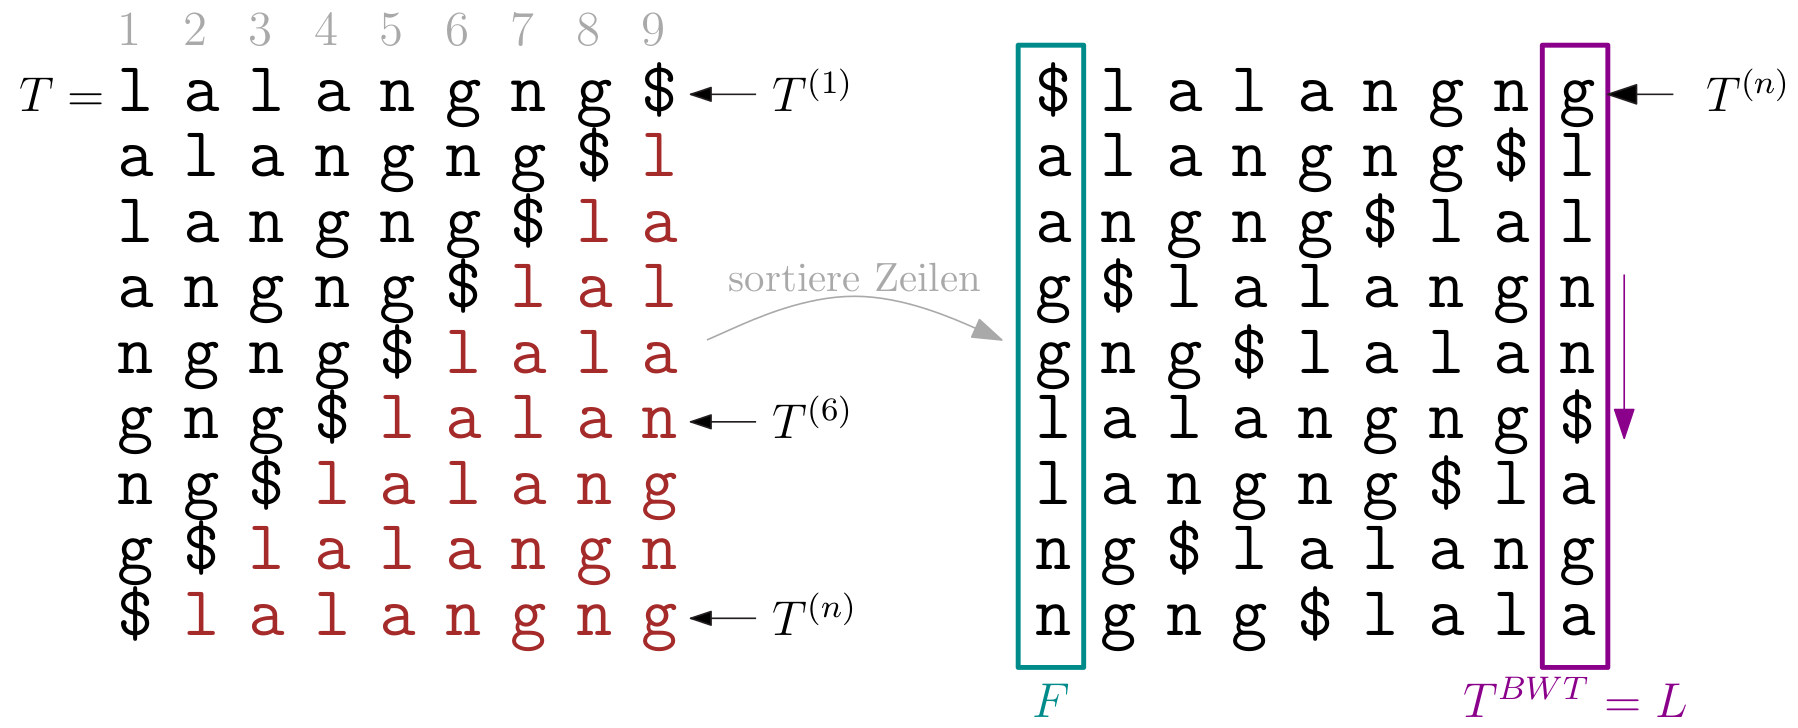
\includegraphics[width=0.7\textwidth]{BWT}
  \caption{Konstruktion der Burrows-Wheler-Transformation von \( T = \texttt{lalalangng\$}  \), \( T^{\text{BWT}} = \texttt{gllnn\$ aga} \). Da \( T^{\text{BWT}} \) die letzte Spalte ist schreibt man oft auch \( L \) stattdessen. Die erste Spalte wird auch \( F \) genannt}
\end{figure}

Naiv benötigt die Berechnung von \( T^{\text{BWT}} \) \( O(n^2 + n\log n) \) Schritte. Die Berechnungszeit lässt sich aber auf \( O(n) \) reduzieren.

\section{Beobachtungen}

Folgende Eigenschaften lassen sich feststellen:

\begin{itemize}
  \item Die Zeilen der oben konstruierten Matrix enthalten die sortierten Suffixe von \( T \) (vom Zeilenstart bis \$ gehend).
  \item Die Zeichen der letzten Spalte (also \( T^{\text{BWT}} \)) sind also die Zeichen, die vor dem zu ihrer Zeile gehörenden Suffix stehen. Formaler ist \( T^{\text{BWT}}[i] \) das Zeichen vor dem \( i \)-ten Suffix in \( T \):
  \begin{equation*}
    T^{\text{BWT}}[i] = L[i] = T[\text{SA}[i]-1] = T^{(\text{SA}[i])}[n]
  \end{equation*}
  Da wir mithilfe des \hyperref[sec:SALinear]{DC3-Algorithmus} das Suffix-Array in Linearzeit berechnen können, können wir auch die Burrows-Wheeler-Transformation in Linearzeit bestimmen.
\end{itemize}

\section{Rücktransformation}

\begin{minipage}{0.8\textwidth}
  Wir können aus einer vorliegenden \( T^{\text{BWT}} \) einfach \( F \) --- also die erste Spalte der Matrix --- konstruieren, indem wir die Buchstaben von \( T^{\text{BWT}} \) sortieren. Hängen wir nun \( T^{\text{BWT}} \) und \( F \) hintereinander, so haben wir bereits Buchstabenpaare, die so auch in \( T \) auftreten. Sortieren wir nun die beiden Spalten (also die Buchstabenpaare) lexikographisch, so erhalten wir die auf \( F \) folgende Spalte. Durch diesen Prozess lässt sich die gesamte Matrix und somit \( T \) rekonstruieren.
\end{minipage}
\hfill
\begin{minipage}{0.15\textwidth}
  \begin{figure}[H]
    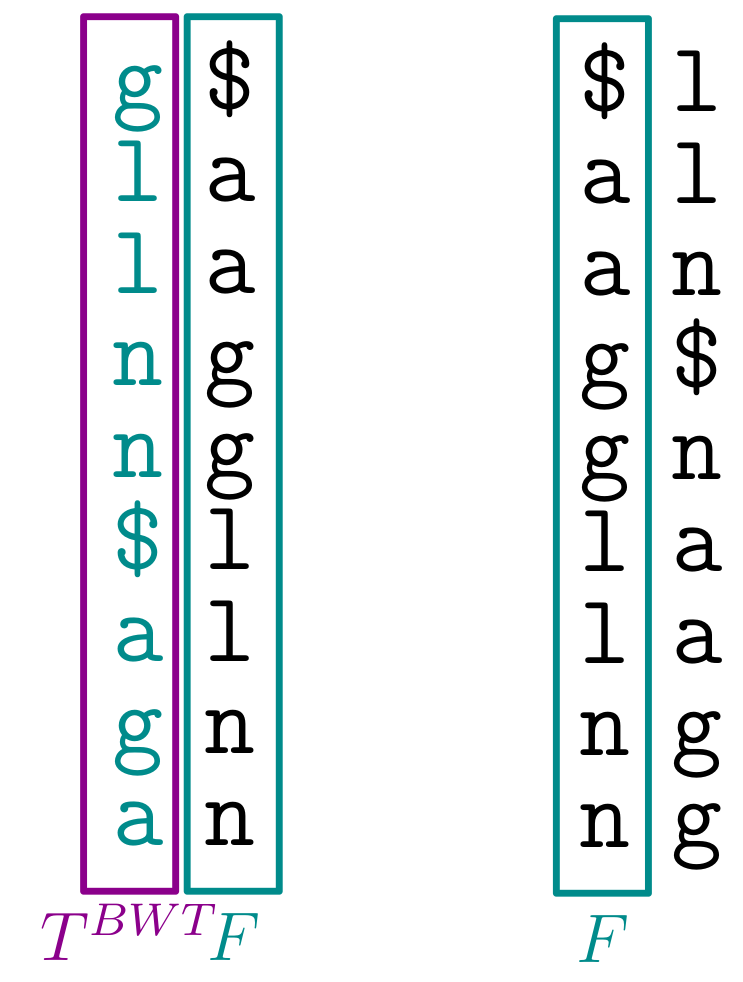
\includegraphics[width=\textwidth]{BWTSorting}
  \end{figure}
\end{minipage}

\clearpage

Diese Art der Rücktransformation benötigt \( O(n^2\log n) \) Schritte. Im Folgenden werden wir die Rücktransformation auf Linearzeit reduzieren. Dazu benötigen wir \term{Last-to-front mapping}\index{Last-to-front mapping}:
\begin{equation*}
  \text{LF}[i] \coloneqq \text{ Position in } L\text{, an der Vorgänger von } L[i] \text{ steht}
\end{equation*}

\begin{minipage}{.65\textwidth}
  Da die Spalten der BWT-Matrix zyklisch sind, ist der Vorgänger von \( L[i] \) derjenige Buchstabe, der in \( F[i] \) steht, also
  \begin{equation*}
    \text{LF}[i] = \text{Position, an der } L[i] \text{ in } F \text{ steht}
  \end{equation*}
\end{minipage}
\hfill
\begin{minipage}{.3\textwidth}
  \begin{figure}[H]
    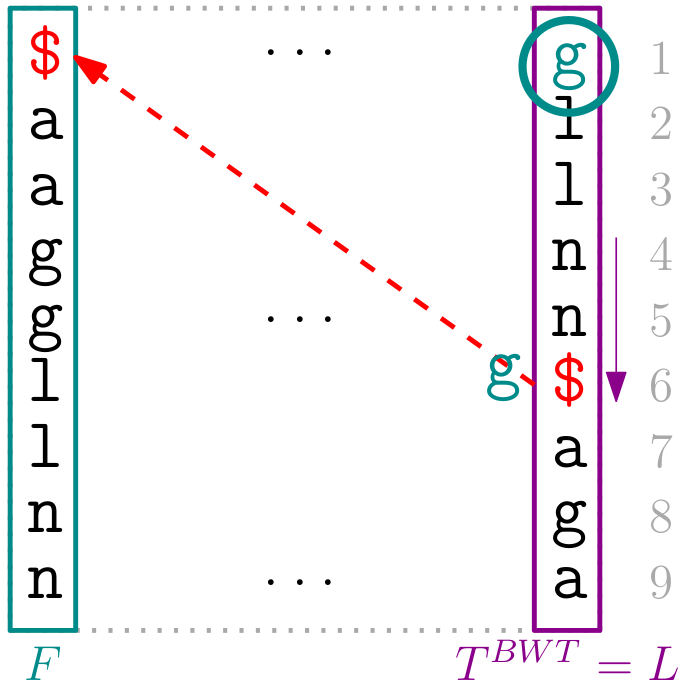
\includegraphics[width=\textwidth]{BWTLF}
    \caption{Gesucht ist der Vorgänger von \texttt{\$}. Stellen wir uns \( T^{\text{BWT}} \) ein zweites Mal links von \( F \) vor, so sehen wir, dass es \texttt{g} ist}
  \end{figure}
\end{minipage}

Wir erhalten folgenden Zusammenhang:
\begin{equation*}
  \text{LF}[i] = j \Leftrightarrow T^{(\text{SA}[j])} = {\left( T^{(\text{SA}[i])} \right)}^{(n)}\text{.}
\end{equation*}

\subsection{Weitere Überlegungen zur Rücktransformation}

Wir können desweiteren folgende Beobachtungen an \( T^{\text{BWT}} \) machen:

\begin{minipage}{.6\textwidth}
  \begin{itemize}
    \item Gleiche Zeichen haben gleiche Reihenfolge in \( F \) und \( L \).
    \item Falls \( L[i] = L[j] \) für \( i < j \), dann ist \( \text{LF}[i] < \text{LF}[j] \).
  \end{itemize}
  Grund dafür ist, dass die Zeilen der BWT-Matrix lexikographisch sortiert sind.
\end{minipage}
\hfill
\begin{minipage}{.35\textwidth}
  \begin{figure}[H]
    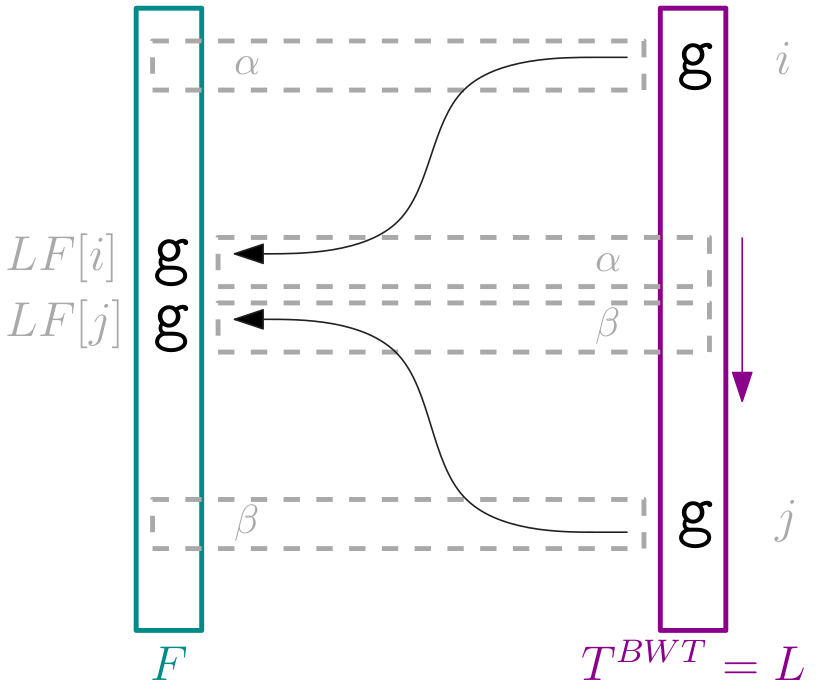
\includegraphics[width=\textwidth]{BWTBack}
    \caption{Präfixe \( \alpha \) und \( \beta \) und wie sie in der Matrix vorkommen}
  \end{figure}
\end{minipage}

Wir können also \( LF \) rein aus \( T^{\text{BWT}} \) berechnen. Dazu brauchen wir nur zwei Hilfsfunktionen:

\begin{itemize}
  \item \( C(a) \coloneqq \# \) Zeichen \( < a \)
  \item \( \text{occ}[i] \coloneqq \# \) Zeichen \( = L[i] \) in \( L[1\dots i] \)
\end{itemize}

Nun können wir \( \text{LF}[i] \) darstellen als
\begin{equation*}
  \text{LF}[i] = C(L[i]) + \text{occ}[i]
\end{equation*}
und können somit \( \text{LF} \) in \( O(n) \) berechnen, da sich \( C \) und \( \text{occ} \) in Linearzeit berechnen lassen.

\subsection{Implementierung}

Zuerst berechnen wir LF. Hier sieht die Implementierung so aus:

\begin{enumerate}
  \item Initialisiere occ und \( h \). \( h \) sei ein Array, das zählt, wie oft ein bestimmter Buchstabe vorkommt, damit wir nachher \( C \) gescheit berechnen können.
  \item Laufe durch \( L = T^{\text{BWT}} \) (\( i = 1 \dots n \))
  \begin{itemize}
    \item \( h(L[i]) \)++
    \item \( \text{occ}(L[i]) = h(L[i]) \)
  \end{itemize}
  \item Konstruiere \( C \) aus \( h \): \( C(\texttt{\$}) = 0 \), \( C(\alpha) = C(\alpha - 1) + h(\alpha - 1) \) (\( \alpha \) ist ein Buchstabe, \( \alpha - 1 \) sein Vorgänger)
  \item \( \text{LF}[i] = C(L[i]) + \text{occ}[i] \)
\end{enumerate}

\begin{figure}[H]
  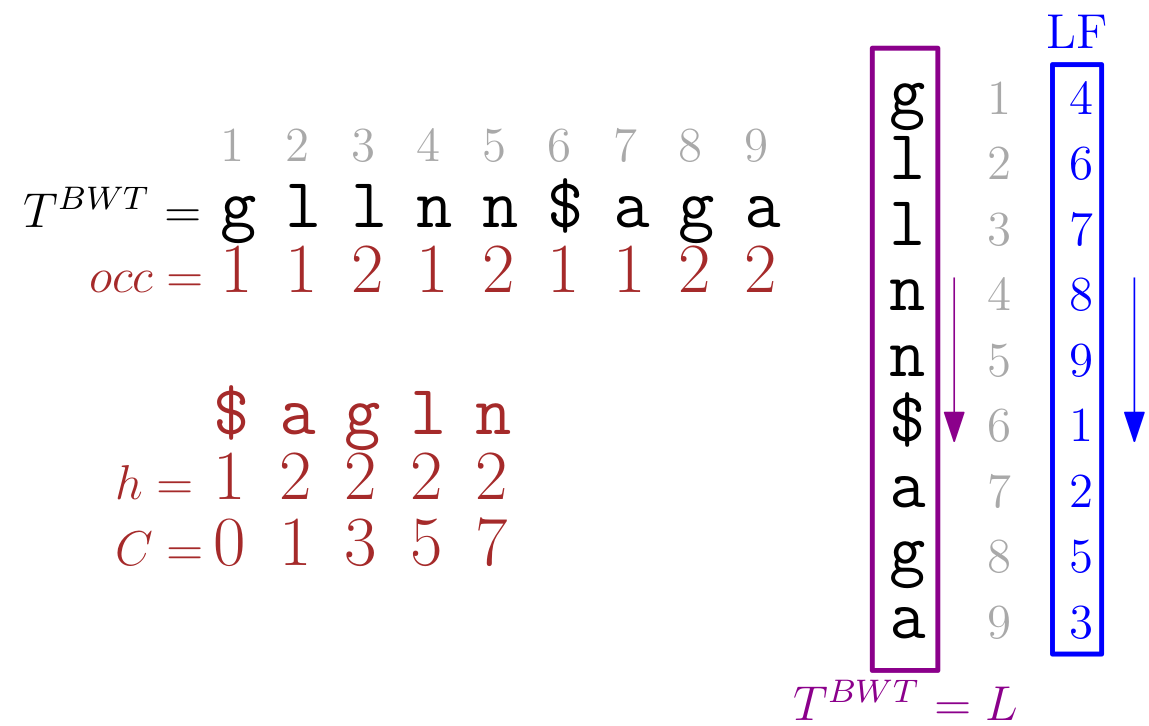
\includegraphics[width=0.6\textwidth]{BWTBackLinear}
  \caption{Beispiel des Algorithmus zur Berechnung von LF nach Durchführung}
\end{figure}

\begin{minipage}{.8\textwidth}
  Nun kann \( T \) von rechts nach links berechnet werden:
  \begin{enumerate}
    \item \( T[n] = \texttt{\$} \Rightarrow \text{LF}[\cdot] = 1 \). Das ist unabhängig von \( T \) so.
    \item \( L[1] = \texttt{g} \Rightarrow T[n-1] = \texttt{g} \Rightarrow \text{LF}[1] = 4 \)
    \item \( L[4] = \texttt{n} \Rightarrow T[n-2] = \texttt{n} \Rightarrow \cdots \)
  \end{enumerate}
  Also geht auch die Rücktransformation in \( O(n) \).
\end{minipage}
\hfill
\begin{minipage}{.15\textwidth}
  \begin{figure}[H]
    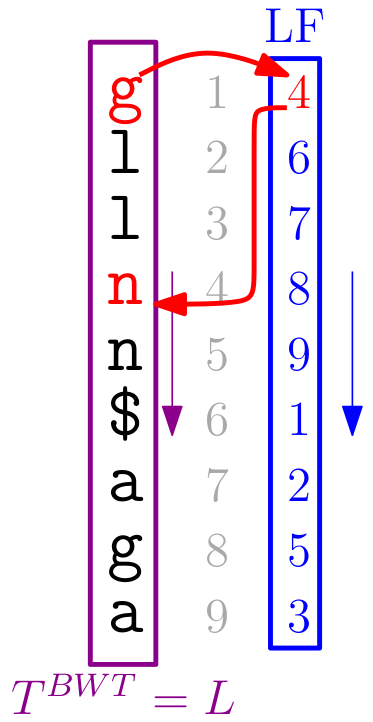
\includegraphics[width=\textwidth]{BWTBackResult}
  \end{figure}
\end{minipage}

\section{Was bringt die BWT?}

Die Vorteile der Burrows-Wheeler-Transformation sind nicht direkt erkennbar --- sie nutzt dieselben Zeichen wie \( T \) und benötigt den gleichen Platz.

Allerdings wird die \emph{Komprimierung stark vereinfacht}, weil Zeichen mit ähnlichem Kontext gruppiert werden. Besonders gut funktioniert sie auf Texten mit vielen gleichen Substrings, wie beispielsweise einem englischen Fließtext. Zur Vereinfachung von \emph{Indexierung} und \emph{Suche} steuert sie auch bei, weil Vorgänger von Suffixen einfach bestimmt werden können.

Im Folgenden werden wir uns die Burrows-Wheeler-Transformation im Kontext von \emph{Kompression} und \emph{Suche} anschauen.

\section{Kompression}

Wir schauen uns zwei Kompressionsmöglichkeiten an: die \emph{move to front}-Kodierung und die Huffman-Kodierung

\subsection{MTF-Kodierung}

Idee der \term{MTF-Kodierung}\index{Kodierung!MTF} ist es, lokale Redundanz zu nutzen und so kleine Zahlen für gleiche Zeichen, die nahe beieinander liegen, zu verwenden. Die Umsetzung funktioniert so:

\begin{enumerate}
  \item Initialisiere \( Y \) mit Alphabet von \( T^{\text{BWT}} \).
  \item Durchlaufe \( T^{\text{BWT}} \) (\( i = 1,\dots,n \))
  \begin{itemize}
    \item Generiere \( R[1,\dots,n] \), wobei \( R[i] \) die Position von \( T^{\text{BWT}}[i] \) in \( Y \) codiert.
    \item Schiebe \( T^{\text{BWT}}[i] \) an den Anfang von \( Y \).
  \end{itemize}
\end{enumerate}

\begin{figure}[H]
  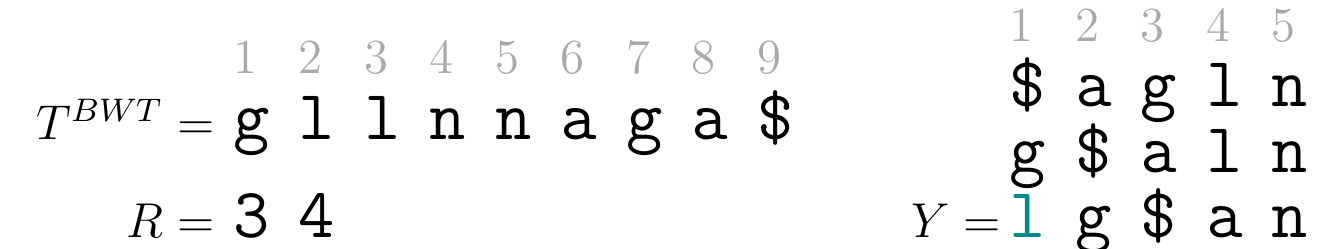
\includegraphics[width=0.8\textwidth]{MTF}
  \caption{Es wurde hier gerade die \texttt{4} eingefügt und deswegen \texttt{l} in \( Y \) nach vorne genommen. Als nächstes muss \texttt{l} codiert (\( \cong \texttt{1} \)) und \( Y \) anschließend nicht verändert werden, weil \texttt{l} ja eh schon ganz vorne steht}
\end{figure}

\clearpage

\subsection{Huffman-Kodierung}

Die \term{Huffman-Kodierung}\index{Kodierung!Huffman} erzeugt präfixfreie Codes variabler Länge. Der Ablauf ist:

\begin{enumerate}
  \item Notiere vorkommende Symbole und ihre jeweiligen Häufigkeiten. Sie sind die Blätter des (binären) Huffman-Baumes.
  \item Verknüpfe die zwei seltenstem Knoten in einem neuen Knoten. Die Häufigkeit des neuen Knotens ist die Summe der Häufigkeiten seiner Kinder. Dies erfolgt nun iterativ.
  \item Die Wurzel hat relative Häufigkeit \( 1 \) (bzw.\ absolute Häufigkeit \( \left\vert T \right\vert \)).
  \item Beschrifte die Kanten zwischen einem Knoten und seinen beiden Kindern mit \( 0 \) und \( 1 \). Der Pfad von der Wurzel zu einem bestimmten Blatt ergibt den Code des Symbols, zu dem das Blatt gehört.
\end{enumerate}

\begin{figure}[H]
  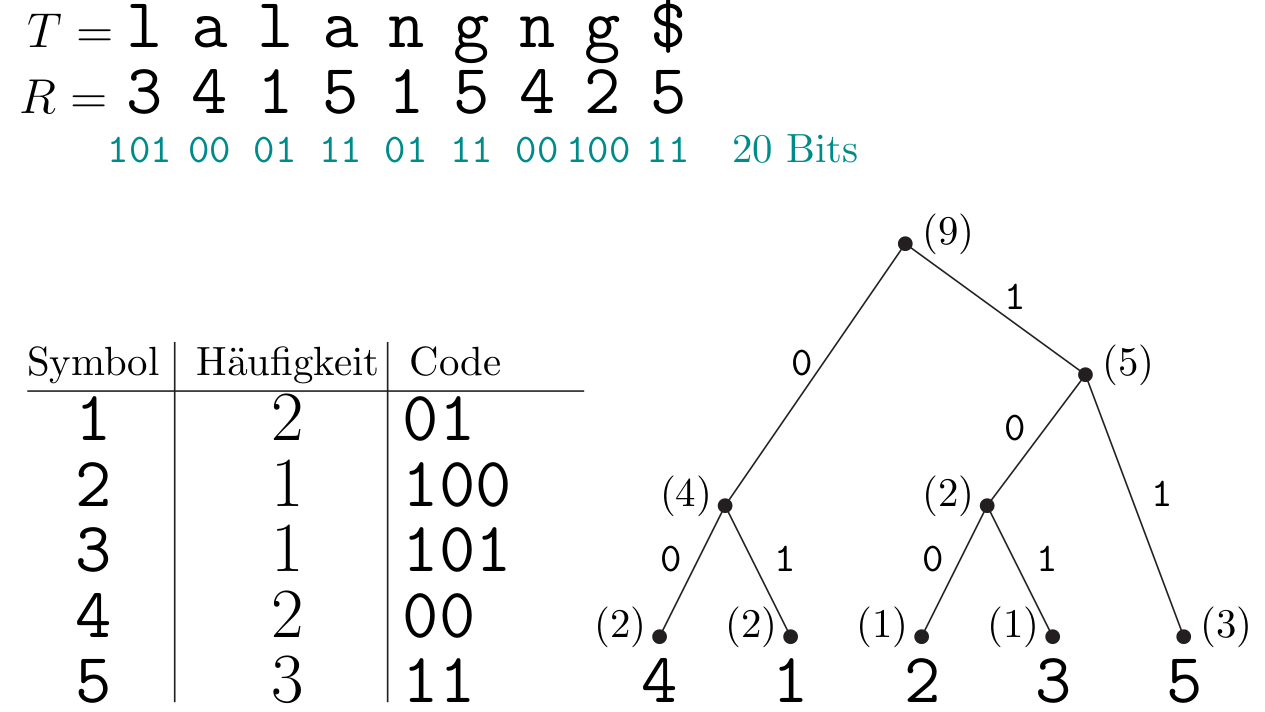
\includegraphics[width=0.6\textwidth]{Huffman}
  \caption{MTF-Kodierung \( R \) von \( T \), die Häufigkeit der in \( R \) vorkommenden Symbole und die mit dem Huffman-Baum erzeugten Codes}
\end{figure}

\section{Suche in der Burrows-Wheeler-Transformation}

Wir möchten nun in \( T^{\text{BWT}} \) nach einem Pattern \( P \) suchen. Hier sei
\begin{align*}
  P &= \texttt{bar} \quad \text{und} \\
  T &= \texttt{abracadabrabarbara\$}\quad\text{und somit} \\
  \text{BWT} &= \texttt{arrd\$rcbbraaaaaabba}
\end{align*}
Wir benötigen dazu zwei Hilfsmittel:

\begin{itemize}
  \item Das Array \( C \) beinhalte für jeden eindeutigen Buchstaben in \( t \in T \) die Position des ersten Suffixes im Suffix-Array, das mit \( t \) beginnt.
  \item \( \text{rank}(i,X,\text{ BWT}) \) gibt an, wie oft ein Buchstabe \( X \) in \( \text{BWT}[0,\dots,i-1] \) vorkommt.
\end{itemize}

Wir suchen nun nach \( P \) in BWT. Wir suchen rückwärts, starten also mit ``\texttt{r}''. Dazu ermitteln wir alle Suffixe, die mit \texttt{r} starten. Wir nutzen dazu \( C \) und rank:

\begin{itemize}
  \item Initiales Intervall: \( [\text{sp}_0, \text{ep}_0] = [0,\dots,n-1] \).
  \item Ermittle Intervall der Suffixe, die mit \texttt{r} starten:
  \begin{itemize}
    \item \( \text{sp}_1 = C[r] + \text{rank}(\text{sp}_0, \texttt{r}, \text{BWT}) = 15 + \text{rank}(0,\texttt{r}, \text{BWT}) = 15+0 = 15 \)
    \item \( \text{ep}_1 = C[r] + \text{rank}(\text{ep}_0 + 1, \texttt{r}, \text{BWT}) - 1 = 15 + 4 - 1 = 18 \)
  \end{itemize}
\end{itemize}

\begin{minipage}{.7\textwidth}
  Wir suchen nun analog nach ``\texttt{ar}'', indem wir \( \text{sp}_2 \) und \( \text{ep}_2 \) aus \( \text{sp}_1 \) und \( \text{ep}_1 \) berechnen. Das Ganze dann nochmal für ``\texttt{bar}'' und wir erhalten 9 und 10 als diejenigen Suffixe, die mit \texttt{bar} anfangen.
\end{minipage}
\hfill
\begin{minipage}{.25\textwidth}
  \begin{figure}[H]
    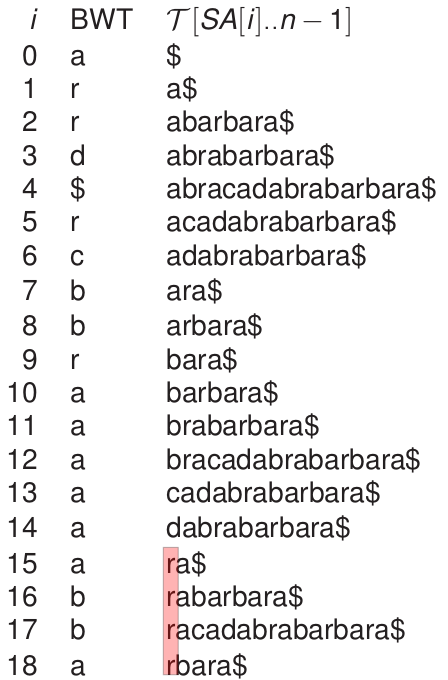
\includegraphics[width=\textwidth]{BWTSearch}
    \caption{Intervall \( [\text{sp}_1, \text{ep}_1] \)}
  \end{figure}
\end{minipage}

\subsection{Zusammenfassung}

Wir brauchen also nur \( C \) und \( R \), um Abfragen zu Existenz und Anzahl eines Patterns machen zu können. Die Ausführungszeit ist in \( O(m*t_{\text{rank}}) \), wobei \( t_{\text{rank}} \) die Ausführungszeit einer rank-Operation ist.

Als nächstes werden wir uns damit beschäftigen, wie wir die rank-Operation implementieren können. Wir werden dazu \emph{wavelet trees}\footnote{Grossi \& Vitter, 2003} verwenden.

\section{Wavelet Trees}

\term{Wavelet Trees}\index{Wavelet Tree} erlauben ein schnelles Berechnen der rank-Operation. Dazu wird in einem Baum codiert, ob ein bestimmter Buchstabe des Strings (hier des BWT) in der oberen oder der unteren Hälfte des Alphabets liegt. So werden die Buchstaben des BWT einem Kindknoten zugeordnet, wo auf dem jeweiligen Teilalphabet erneut eine Zweiteilung stattfindet. Dieser Prozess wiederholt sich so lange, bis in jedem Blatt nur Zeichen einer Art stehen.

\begin{figure}[H]
  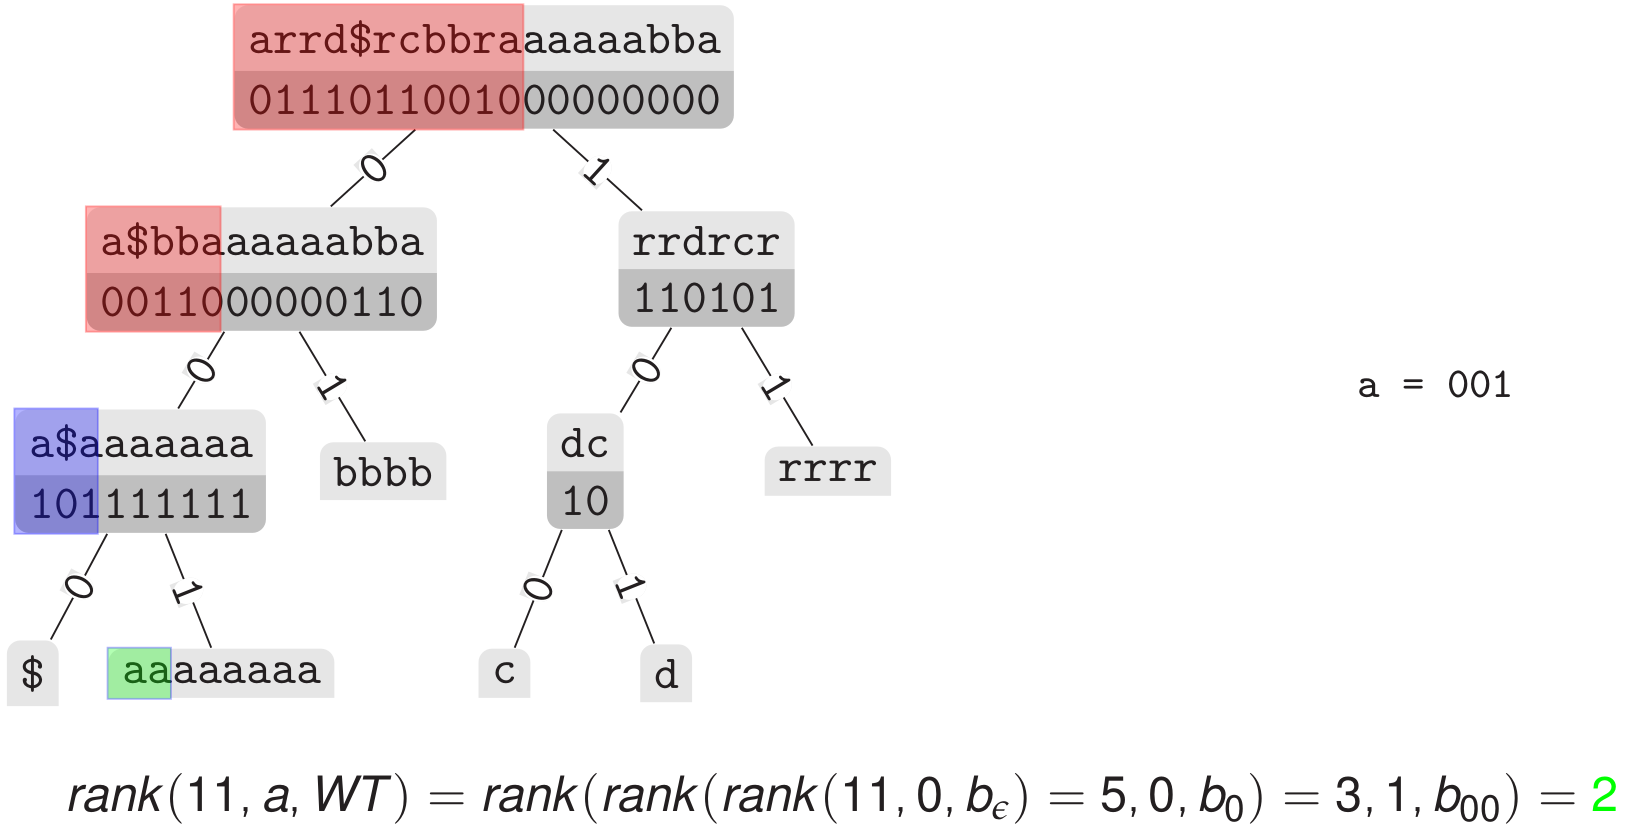
\includegraphics[width=0.8\textwidth]{WaveletTree}
  \caption{Wavelet Tree einer BWT und zugehörige Berechnung von \( \text{rank}(11, \textsc{a}, \text{BWT}) \)}
\end{figure}

Abfragen können auf einem Wavelet Tree in konstanter Zeit durchgeführt werden. Der Wavelet Tree selbst benötigt \( o(n) \) viel Platz, genauer
\begin{equation*}
  O\left( \frac{n}{\log n} + \frac{n \log \log n}{\log n} + \sqrt{n}\log n \log\log n \right)\text{.}
\end{equation*}

Die Konstruktion des Wavelet-Trees ist nicht zwingend an die Unterteilung des BWT zwei lexikographische Teilalphabete gebunden. Beispielsweise lässt sich eine Unterteilung in zwei Teilwörter auch durch die Häufigkeit der Buchstaben konstruieren, wodurch ein \term{Huffman-Wavelet-Tree}\index{Wavelet Tree!Huffman} entsteht.

\section{Exkurs --- Succinct Data Structures}

\textcolor{red}{\textbf{Hinweis}}: Dieser Abschnitt ist \emph{nicht} klausurrelevant!

\ \\

Eine extrem platzeffiziente Datenstruktur, \term{succinct data structure}\index{succinct data structure} genannt, benötigt nur wenig mehr Platz als die informationstheoretische untere Grenze, unterstützt allerdings Operationen zeiteffizient.

Sei \( L \) die informationstheoretische untere Schranke, die zur Repräsentierung einer Klasse von Objekten benötigt wird. Eine Datenstruktur, die Operationen trotzdem zeiteffizient unterstützt, heißt
\begin{itemize}
  \item \emph{implicit}, falls sie \( L + O(1) \) Bits Platz braucht (also nur konstant mehr als die informationstheoretische untere Schranke, z.B. Heap),
  \item \emph{succinct}, falls sie \( L + o(L) \) Bits Platz braucht (also nur sublinear mehr als die informationstheoretische untere Schranke, z.B. Baum),
  \item \emph{compact}, falls sie \( O(L) \) Bits Platz braucht. 
\end{itemize}

\subsection{Binärbäume --- succinct}

Es gibt \( C_n = \frac{1}{n+1}\binom{2n}{n} \) Binärbäume auf \( n \) Knoten. Um einen Binärbaum auf \( n \) Knoten speichern zu können, brauchen wir \( \log C_n = 2n + o(n) \) bits.\footnote{Das kann mithilfe der Sterling-Approximation gezeigt werden.} Wir wollen folgende Operationen unterstützen:
\begin{itemize}
  \item \( \text{parent}(v) \)
  \item \( \text{leftchild}(v) \)
  \item \( \text{rightchild}(v) \)
\end{itemize}

Eine mögliche Kodierung wäre, zu jedem Knoten des Baumes, der kein Blatt ist, so viele imaginäre Knoten hinzuzufügen, dass der jeweilige Knoten zwei Kinder hat (also entweder, 0, 1 oder 2 imaginäre Knoten). Diesen Prozess führt man durch, bis alle Blätter des Baumes dieselbe Tiefe haben. Wir können nun alle Knoten durchnummerieren und pro Knoten in einem Bit-Array speichern, ob der Knoten real (=1) ist oder nicht (=0).

\begin{figure}[H]
  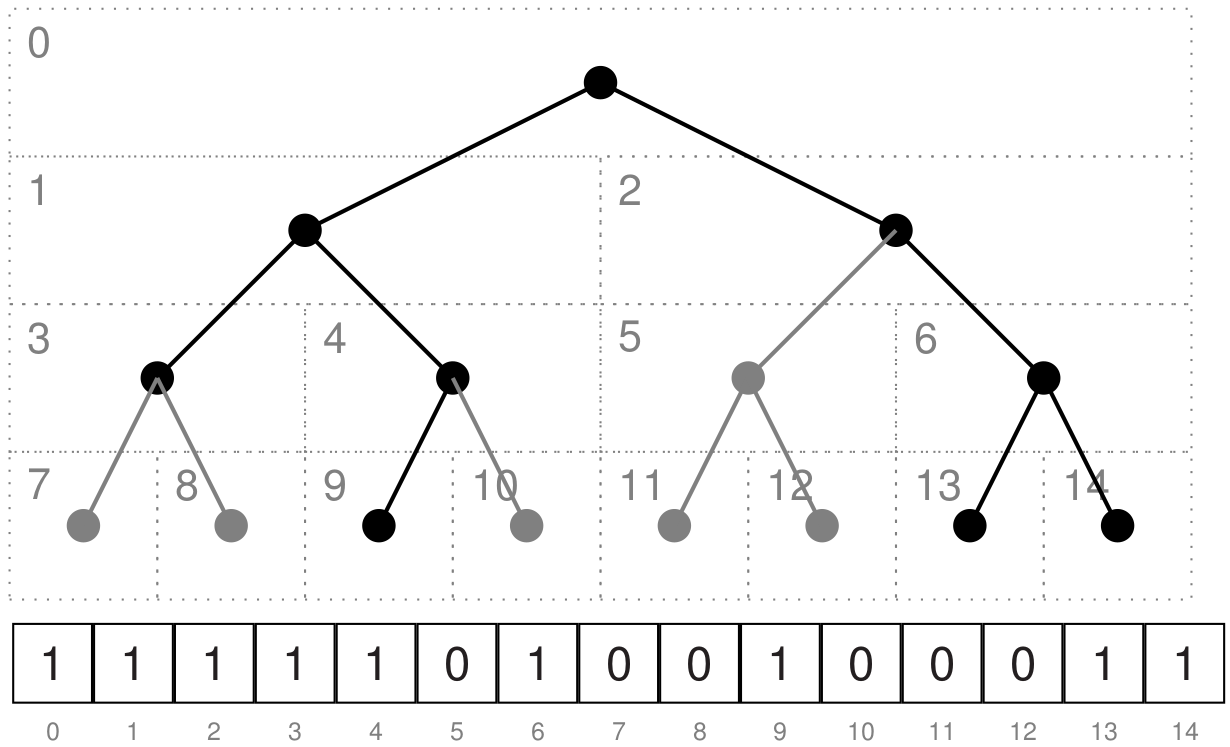
\includegraphics[width=0.5\textwidth]{SuccinctBinaryTree}
  \caption{Die schwarzen Knoten sind die realen Knoten des Baumes, die grauen die imaginären}
\end{figure}

Die geforderten Operationen können hier sehr einfach implementiert werden:
\begin{itemize}
  \item \( \text{parent}(v) = \left\lfloor \frac{v-1}{2} \right\rfloor \) (für \( v \neq \) Wurzel)
  \item \( \text{leftchild}(v) = 2v + 1 \)
  \item \( \text{rightchild}(v) = 2v + 2 \)
\end{itemize}

Problem dieses Ansatzes ist, dass für einen Binärbaum mit einer Maximaltiefe \( d \) stets \( 2^d \) Bits benötigt werden.

Jacobson schlug 1989 einen besseren Algorithmus vor:

\begin{enumerate}
  \item Alle Knoten des Binärbaums mit \( 1 \) markieren.
  \item Kinder jedes Knotens im Baum mit imaginären Knoten auf \( 2 \) ergänzen.
  \item Bit-Markierungen wie im vorhergehenden Algorithmus ablesen.
\end{enumerate}

Benötigt wird eine weitere Operation \( \text{rank}(i, \texttt{type}, b) \), die für Knoten \( i \) des ergänzten Baums \( b \) zurückgibt, um den wievielten Knoten des Typs \texttt{type} es sich handelt. Wir erhalten folgendes Resultat:

\begin{figure}[H]
  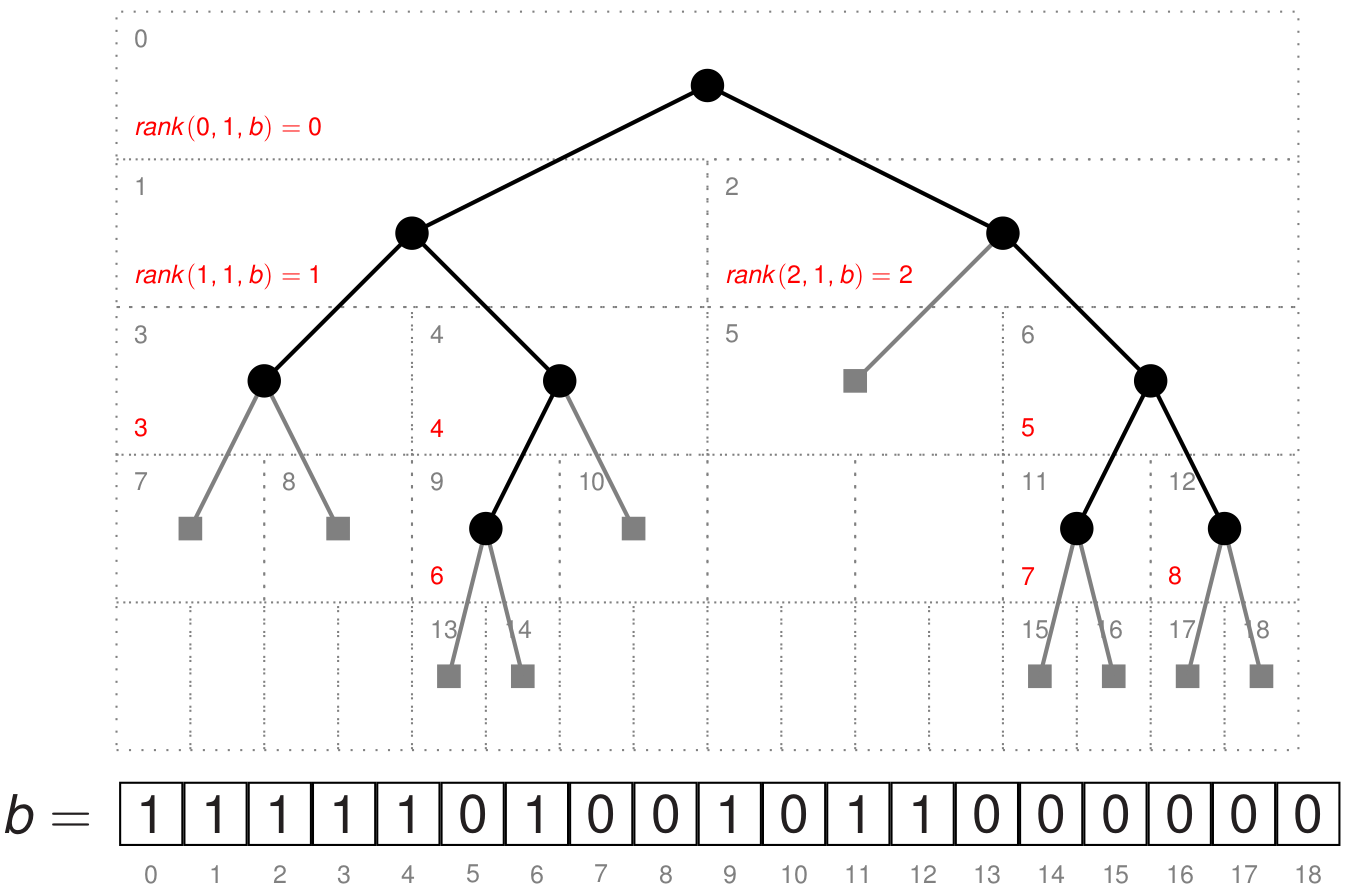
\includegraphics[width=.6\textwidth]{SuccinctBinaryTree2}
  \caption{Jacobson-Kodierung eines Binärbaums}
\end{figure}

Wir können hiermit also einen Binärbaum mit einem Bit-Array der Länge \( 2n + 1 \) (mit \( n \) gesetzten Bits) repräsentieren. Die gewünschten Operationen funktionieren hier so:

\begin{itemize}
  \item \( \text{leftchild}(v) = 2\text{rank}(v) + 1 \)
  \item \( \text{rightchild}(v) = 2\text{rank}(v) + 2 \)
  \item \( \text{parent}(v) =  \) auch in konstanter Zeit möglich\footnote{Übungsaufgabe!}
\end{itemize}

Der totale Platzverbrauch inklusive rank ist also \( 2n + o(n) \) Bits.


\subsection{Bäume --- succinct: LOUDS}

Die Abkürzung \emph{LOUDS} steht für \term{level order unary degree sequence}\index{LOUDS}.

Die Implementierung funktioniert so:

\begin{enumerate}
  \item Füge über der Wurzel des Baums eine Pseudo-Wurzel hinzu und verbinde sie nur mit der alten Wurzel.
  \item Der Ausgangsgrad wird zu jedem Knoten unär\footnote{Ausgangsgrad \( x \): \( x \) mal \texttt{0}, hintendran immer noch eine \texttt{1}.} codiert dazugeschrieben.
\end{enumerate}

Die \term{LOUDS-Sequenz}\index{LOUDS!Sequenz} ist nun die Konkatenantion der Knotenmarkierungen (sortiert nach Level).

\begin{figure}[H]
  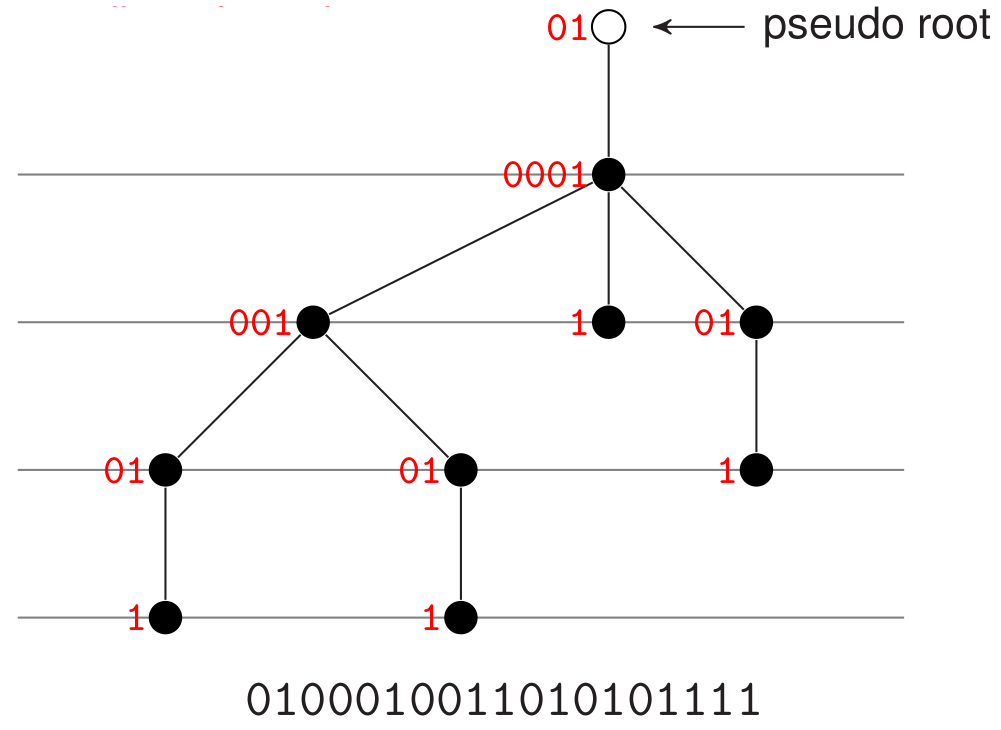
\includegraphics[width=0.5\textwidth]{LOUDS}
  \caption{Allgemeiner Baum mit Pseudo-Wurzel, Knotenmarkierungen und LOUDS-Sequenz}
\end{figure}

Die Konstruktion verursacht, dass --- abgesehen von der Wurzel --- jeder Knoten zweimal in der LOUDS-Sequenz vorkommt: einmal als \texttt{0} in der Kinder-Liste seines Elternknotens und einmal als terminierende \texttt{1} in seiner eigenen Kinder-Liste.

Der gesamte Platzverbrauch hiervorn ist \( 2n + 1 + o(n) \) Bits. Außerdem lassen sich alle gewünschten Operationen in konstanter Zeit implementieren:

\ \\ 

\begin{minipage}{.475\textwidth}
  \begin{pseudocode}
    \textbf{\textsc{isLeaf}}\( (v) \) \\
    id \( \coloneqq \text{rank}(v, 0, \text{LOUDS}) \) \\
    \( p \coloneqq \text{select}(\text{id} + 2, 1, \text{LOUDS}) \) \\
    \textbf{return} \( \text{LOUDS}[p-1] == 1 \) \\
  \end{pseudocode}
\end{minipage}
\hfill
\begin{minipage}{.475\textwidth}
  \begin{pseudocode}
    \textbf{\textsc{outDegree}}\( (v) \) \\
    \textbf{if} \textsc{isLeaf}\( (v) \) \textbf{then return} \( 0 \) \\
    \( \text{id} \coloneqq \text{rank}(v,0,\text{LOUDS}) \) \\
    \textbf{return} \( \text{select}(\text{id}+2,1,\text{LOUDS}) - \) \\ \phantom{\textbf{return}} \( \text{select}(\text{id} + 1, 1, \text{LOUDS}) - 1 \)
  \end{pseudocode}
\end{minipage}

\begin{minipage}{.475\textwidth}
  \begin{pseudocode}
    \textbf{\textsc{child}}\( (v,i) \) \\
    \textbf{if} \( i < \textsc{outDegree}(v) \) \textbf{then} \\ \phantom{\enskip} \textbf{return} \( \perp \) \\
    \( \text{id} \coloneqq \text{rank}(v,0,\text{LOUDS}) \) \\
    \textbf{return} \( \text{select}(\text{id} + 1, 1, \text{LOUDS}) + i \)
  \end{pseudocode}
\end{minipage}
\hfill
\begin{minipage}{.475\textwidth}
  \begin{pseudocode}
    \textbf{\textsc{parent}}\( (v) \) \\
    \textbf{if} \( \textsc{isRoot}(v) \) \textbf{then} \\ \phantom{\enskip} \textbf{return} \( \perp \) \\
    \( \text{pid} \coloneqq \text{rank}(v,1,\text{LOUDS}) \) \\
    \textbf{return} \( \text{select}(\text{pid},0,\text{LOUDS}) \)
  \end{pseudocode}
\end{minipage}